% standard
\documentclass[a4paper,12pt]{article}
\usepackage[utf8]{inputenc}
\usepackage[ngerman]{babel}

% geometry
\usepackage{geometry}
\geometry{ headsep=20pt,
headheight=20pt,
left=21mm,
top=15mm,
right=21mm,
bottom=15mm,
footskip=20pt,
includeheadfoot}

% header and footer
\usepackage{datetime}
\newdateformat{dmy}{%
\THEDAY.~\monthname[\THEMONTH] \THEYEAR}
\usepackage{fancyhdr}
\pagestyle{fancy}
\lhead{Noah Vogt \& Simon Hammer}
\chead{}
\rhead{\dmy\today}
\lfoot{}
\cfoot{Gymnasium Kirschgarten}
\rfoot{Seite \thepage}
\renewcommand{\footrulewidth}{.4pt}

% fix figure positioning
\usepackage{float}

% larger inner table margin
\renewcommand{\arraystretch}{1.4}

% no paragraph indent
\setlength{\parindent}{0em}

% graphics package
\usepackage{graphicx}

\usepackage{multicol}

% use sans serif font
\usepackage{tgheros}
\usepackage{mathptmx}

% don't even ask what this is for, I have no idea (noah)
\usepackage{bm} %italic \bm{\mathit{•}}
\usepackage[hang]{footmisc}
\usepackage{siunitx}
\usepackage[font={small,it}]{caption}
\sisetup{locale = DE, per-mode = fraction, separate-uncertainty,   exponent-to-prefix, prefixes-as-symbols = false, scientific-notation=false
}
\newcommand{\ns}[4]{(\num[scientific-notation=false]{#1}\pm\num[scientific-notation=false]{#2})\cdot\num[]{e#3}\si{#4}}

% show isbn in bibliography
\usepackage{natbib}

\begin{document}

\begin{titlepage}

\vspace*{1cm}
	\centering
	
	{\scshape\Large Protokolle Praktikum Physik 3cg \par}
	\vspace{0.5cm}
	{\huge\bfseries die experimentelle Bestimmung der Kapazität eines unbekannten Kondensators\par}
	\vspace{0.5cm}
	{\Large Noah Vogt \& Simon Hammer\par}
	\vspace{17cm}

	{\large Durchgeführt am 27. Oktober 2020\par}
	
\end{titlepage}

\tableofcontents
\pagebreak

\section{Versuchsziel}
Ziel ist es die \textit{Kapazität} $C_u$ eines Kondensators mittels eines \textit{Experiments} so genau wie möglich zu bestimmen, indem ein Kondensator, mit bekannter Kapazität, mit einer bestimmten Spannung, aufgeladen wird. Durch ein Zusammenschliessen der beiden Kondensatoren wird der zweite auch aufgeladen, sodass beide Kondensatoren die gleiche Spannung haben (\textit{Spannungsausgleich}). Nun kann mithilfe einiger Formeln die gesuchte Kapazität des unbekannten Kondensators besimmt werden. Vorausschtlich wird der Messwert unter dem realen Wert liegen aufgrund systematischer Fehler.

\section{Physikalischer Hintergrund}

Die Fähigkeit Ladung zu Speichern macht einen Kondesator aus. Die Menge an Ladungsträgern, welche ein Kondensator unter einer gewissen Spannung aufnehmen kann, nennt sich Kapazität. Die Einheit der Kapazität ist Farad also $[C] = 1 $F \\

Die gespeicherte Ladung ist proportional zu der Spannung $Q \mathtt{\sim} U$ , weil es immer schwerer wird, mehr Ladung auf einen Träger zu speichern, desshalb muss die Spannugsquelle mehr Arbeit verrichten. Mit einer geeignete \textit{konstante C} wird nun die Formel vollendet.

$$Q=C\cdot U$$


Der \textit{Kondensator 2} wird aufgeladen und mit einem anderen nicht geladenen Kondensator (Kondensator 1) Parallelgeschalten. 
Nach dem Parallelschalten der beiden Kondensatoren kommt es zu einem Spannungsausgleich. Wobei eine neue konstante Spannung $u'$ der beiden Kondensatoren entsteht. Durch Umformen der obigen Gleichung gilt

$$\frac{Q_1}{C_u} = \frac{Q_2}{C_b} = u'\quad \Rightarrow \quad Q_2 = u' \cdot C_b \quad , \quad C_u = \frac{Q_1}{u'} $$

Die Totale Ladung berechnet sich aus der Kapazität des zuerst aufgeladenen Kondensators (\textit{Kondensator 2}) und der   Spannung vor dem Parallelschalten, weil nach dem aufladen jenes Kondensators kein neuer Strom dem System hinzugefügt wird und  idealisiert nicht mit einem Stromverbrauch gerechnet wird. Ebenso ergibt sich die Totale Ladung des Systems aus der Ladungen der einzelnen Kondensatoren nach dem parallelschalten. Somit folgt:

$$Q_{Total} = C_b \cdot u$$

$$Q_{Total} = Q_1+Q_2 \quad \Rightarrow \quad Q_1=Q_{Total}-Q_2$$

Durch umformen und einsetzen ergibt sich dann:

$$C_u = \frac{Q_1}{u'} = \frac{Q_{Total}-Q_2}{u'} = \frac{C_b \cdot u - u' \cdot C_b}{u'}$$

\section{Versuchsaufbau}
\begin{figure}[H]

\centering
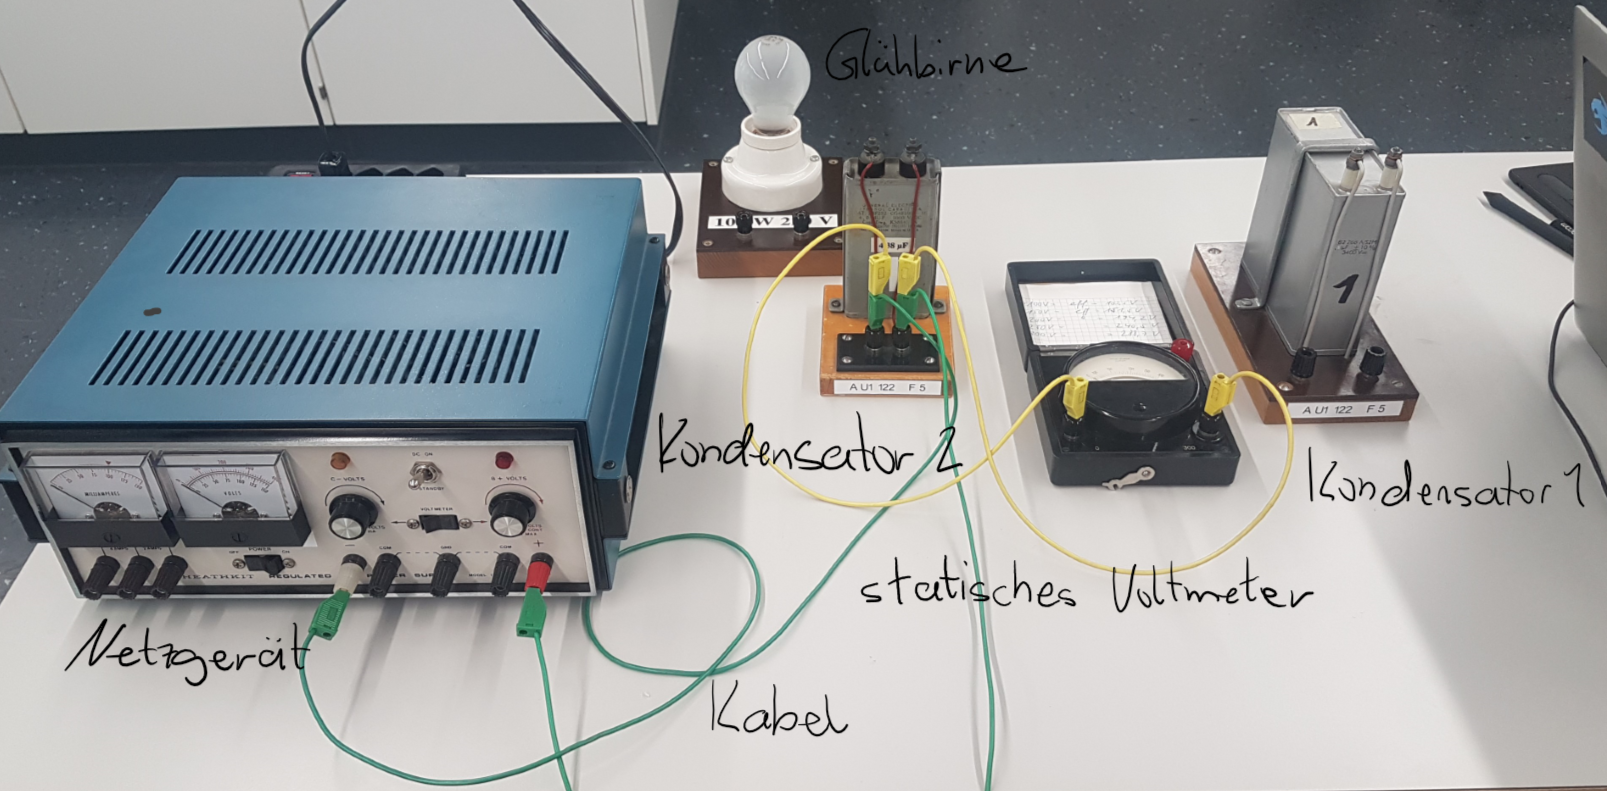
\includegraphics[width=.8\textwidth]{media/bennenung.png}

\end{figure}

\section{Versuchsdurchführung}
\begin{table}[H]
    \centering
    \begin{tabular}{|c|c|c|}
        \hline
        \textbf{Beschreibung} & \textbf{Abkürzung} & \textbf{Wert} \\
        \hline
        Kapazität bekannter Kondensator & $C_{b}$ & $(4.38\pm 0.005 )\mu F$\\
        \hline
        Spannung bekannter Kondensator 1 & $u_{1}$ & $(260\pm 2.5)V$\\
        Spannung bekannter Kondensator 2 & $u_{2}$ & $(300\pm 2.5)V$\\
        Spannung bekannter Kondensator 3 & $u_{3}$ & $(280\pm 2.5)V$\\
        \hline
        Spannung nach dem Ausgleich 1 & $u_{1}'$ & $(178\pm 2.5)V$\\
        Spannung nach dem Ausgleich 2 & $u_{2}'$ & $(201\pm 2.5)V$\\
        Spannung nach dem Ausgleich 3 & $u_{3}'$ & $(192\pm 2.5)V$\\
        \hline
    \end{tabular}
\end{table}
Als erstes wird die Kapazität vom \textit{Kondensator 2} abgelesen und an das Netzgerät mit den Kabeln angeschlossen. Das \textit{statische Voltmeter} wird an den \textit{Kondensator 2} angeschlossen und das Netzgerät wird angeschaltet. Der \textit{Kondensator 2} wird mit einer gewissen Menge Volt geladen, welche beim \textit{Voltmeter} ablesen wird. Die Kabel werden von dem Netzgerät entfernt und direkt, ohne eine berührung mit etwas anderem, in den \textit{Kondensator 1} gesteckt. Die Spannung nimmt ab und wird nochmals gemessen, wenn sie Stabil ist. Nun werden die Kondensatoren einzeln mit der Glühbirne Parallelgeschalten und entladen. Der ganze Vorgang wird dreimal wiederholt mit unterschidlicher ausgangs Spannung. 

\newpage
\section{Versuchsauswertung}

$$C_u = \frac{C_b \cdot u - u' \cdot C_b}{u'}$$

\subsection{Durchführung 1}

$C_{u_{max}} = \displaystyle{\frac{C_{b_{max}}\cdot u_{1_{max}}-u_{1_{min}}'\cdot C_{b_{min}}}{u_{1_{min}}'}}$\\\\

$C_{u_{max}} = \displaystyle{\frac{4.385\cdot 10^{-6}\;F\cdot 262.5\;V-175.5\;V\cdot 4.375\cdot 10^{-6}\;F}{175.5\;V}} = 2.184\cdot 10^{-6}\;F$\\\\

$C_{u_{min}} = \displaystyle{\frac{C_{b_{min}}\cdot u_{1_{min}}-u_{1_{max}}'\cdot C_{b_{max}}}{u_{1_{max}}'}}$\\\\

$C_{u_{min}} = \displaystyle{\frac{4.375\cdot 10^{-6}\;F\cdot 257.5\;V-180.5\;V\cdot 4.385\cdot 10^{-6}\;F}{180.5\;V}} = 1.856\cdot 10^{-6}\;F$\\\\

$\Rightarrow C_{u_1}=\displaystyle{\frac{C_{u_{max}}+C_{u_{min}}}{2}} = 2020052 (\pm 163709)\cdot F = 2.02 (\pm 0.16)\;\mu F$

\subsection{Durchführung 2}

$C_{u_{max}} = \displaystyle{\frac{C_{b_{max}}\cdot u_{2_{max}}-u_{2_{min}}'\cdot C_{b_{min}}}{u_{2_{min}}'}}$\\\\

$C_{u_{max}} = \displaystyle{\frac{4.385\cdot 10^{-6}\;F\cdot 302.5\;V-198.5\;V\cdot 4.375\cdot 10^{-6}\;F}{195.5\;V}} = 2.343\cdot 10^{-6}\;F$\\\\

$C_{u_{min}} = \displaystyle{\frac{C_{b_{min}}\cdot u_{2_{min}}-u_{2_{max}}'\cdot C_{b_{max}}}{u_{2_{max}}'}}$\\\\

$C_{u_{min}} = \displaystyle{\frac{4.375\cdot 10^{-6}\;F\cdot 297.5\;V-203.5\;V\cdot 4.385\cdot 10^{-6}\;F}{203.5\;V}}= 2.011\cdot 10^{-6}\;F$\\\\

$\Rightarrow C_{u_2}=\displaystyle{\frac{C_{u_{max}}+C_{u_{min}}}{2}} = 2176861 (\pm 165977)\cdot F = 2.18 (\pm 0.17)\;\mu F$

\subsection{Durchführung 3}

$C_{u_{max}} = \displaystyle{\frac{C_{b_{max}}\cdot u_{3_{max}}-u_{3_{min}}'\cdot C_{b_{min}}}{u_{3_{min}}'}}$\\\\

$C_{u_{max}} = \displaystyle{\frac{4.385\cdot 10^{-6}\;F\cdot 282.5\;V-189.5\;V\cdot 4.375\cdot 10^{-6}\;F}{189.5\;V}}$\\\\

$C_{u_{min}} = \displaystyle{\frac{C_{b_{min}}\cdot u_{3_{min}}-u_{3_{max}}'\cdot C_{b_{max}}}{u_{3_{max}}'}}$\\\\

$C_{u_{min}} = \displaystyle{\frac{4.375\cdot 10^{-6}\;F\cdot 277.5\;V-194.5\;V\cdot 4.385\cdot 10^{-6}\;F}{194.5\;V}}$\\\\

$\Rightarrow C_{u_3}=\displaystyle{\frac{C_{u_{max}}+C_{u_{min}}}{2}} = 2009485 (\pm 152519)\cdot F = 2.01 (\pm 0.15)\;\mu F$

\section{Kommentar / Diskussion}

\subsection{Genauigkeit}
-Voltmeter recht ungenau, verbraucht vllt. sogar noch strom

-fehlerschranken

-energie geht verloren ein wenig bei der der parallelschaltung (keine 100\% ige effizienz)

-(wärme geht an umwelt verloren)

Bei den beiden Versuchsdurchgängen wurden beim ersten Mal eine Abweichung von \textit{13\%} und beim zweiten Mal \textit{37\%} festgestellt.\\

Aufgrund der vielen systematischen Fehler, da nicht in einem abgschlossenen System experimentiert werden konnte, kann die Ungenauigkeit der Messresultate erklärt werden. Der Tabellenwert $\num{3.338 e5}\si{\J\per\kg}$ \cite{formelsammlung} wurde wie erwartet unterschritten, da einige Energie aus unserem System an die Umgebung verloren ging.\\

Es ist noch anzumerken, dass bei der Berechnung keine Fehlerschranke bei der Masse gemacht wurde. Dies ist zu begründen, dass diese Ungenauigkeit im Vergleich zur Temperaturmessung vernachlässigbar ist.

\subsection{Fehlerquellen}

Ein systematisch Fehler bestand darin, dass das Kalorimeter nicht zu 100\% isoliert und durch die Wände konstant Energie an die Umwelt abgegeben wird. Vorallem da das Kalorimeter nach oben offen war, entstanden dabei beträchtlich mehr Wärmeverluste am Wasser an die Umgebung als nur den Wänden.\\

Ein weiterer Fehler bestand darin, dass das Eis nicht vollständig mit dem Papier abgetrocknet werden konnte.\\

Beim der zweiten Versuchsdurchführung ist ein kleiner Fehler unterlaufen: Das Eis ist auf den Tisch gefallen und wurde dann mit dem Händen in das Kalorimeter befördert. Dabei ist ein Teil des Eises geschmolzen, weil Wärmeenergie von den Händen an das Eis abgegeben wurde. Somit ist die höhere Abweichung vom Tabellenwert im Vergleich zum ersten Versuchsdurchlauf begründet.

\end{document}
